Die Trusted Execution Environment (TEE) zeichnet sich durch drei wesentliche Eigenschaften aus, die ihre Funktionalität und Sicherheit beschreiben. Sie gewährleistet (1) die Authentizität des ausgeführten Codes, indem sie sicherstellt, dass dieser tatsächlich von der beabsichtigten Quelle stammt und nicht manipuliert wurde.  Sie sichert (2) die Integrität des Codes, indem sie während der Ausführung sicherstellt, dass dieser nicht verändert wurde und sie schützt (3) die Vertraulichkeit von Code, Daten und Laufzeitvariablen, indem sie sicherstellt, dass diese nur von privilegierten Parteien eingesehen werden kann. 

Aufgrund der Interaktion von Programmen innerhalb der TEE und Programmen außerhalb, kann die TEE auch als Kompartiment betrachtet werden. Diese Struktur ermöglicht eine klare Trennung zwischen den unterschiedlichen Kompartiments und ermöglicht so eine bessere Kontrolle über den Zugriff.

\subsection{TEE}
Der genaue Aufbau und das Verhalten von Trusted Execution Environments (TEEs) variieren, lassen sich aber im Allgemeinen in zwei Kategorien einteilen: (1) TEEs, die sich einen Adressraum mit dem unprivilegierten Host teilen, und (2) TEEs, bei denen die CPU konzeptionell in eine normale und eine sichere Welt unterteilt ist.

In der ersten Kategorie hat nur die Enklave selbst vollen Zugriff auf ihren Speicherplatz und kann die Daten im Klartext lesen. Eine Enklave ist ein isolierter Speicherbereich innerhalb einer TEE, der dazu dient, Code und Daten vor unautorisiertem Zugriff und Manipulation zu schützen. Selbst privilegierte Benutzer und das Betriebssystem haben keinen Zugriff auf die innerhalb der Enklave gespeicherten Daten. Programme innerhalb der Enklave dürfen jedoch auch auf den Adressraum außerhalb der Enklave zugreifen.Diese Struktur ermöglicht einen besseren Datenaustausch, birgt jedoch das Risiko unsicherer Speicherzugriffe, was potenziell zu Sicherheitslücken führen kann.

In der zweiten Kategorie ist der Adressraum strikt in zwei separate Bereiche unterteilt, wobei keiner der beiden Bereiche auf den jeweils anderen zugreifen kann. Der Datenaustausch zwischen diesen beiden Welten erfolgt über das Trusted Operating System (TOS). Da das TOS privilegierten Zugriff hat, kann es einen geteilten Adressraum einrichten, in dem Daten sicher ausgetauscht werden können. Diese Methode bietet eine stärkere Isolation und somit ein höheres Maß an Sicherheit, da direkte Speicherzugriffe zwischen der normalen und der sicheren Welt verhindert werden, jedoch auf Kosten der Datenübertragungsraten.

In beiden Kategorien gewährleistet sowohl der Prozessor, dass extern kein Zugriff auf die Daten möglich ist, als auch das TOS, dass der Code in der Enklave sicher ist. Ein weiterer Grundgedanke beim Designen einer TEE ist Angreifermodel. Man entwickelt die TEE unter der Annahme, dass sie in einem System ausgeführt wird, das als kompromittiert betrachtet wird und Angreifer die volle Kontrolle über sämtliche Hardware haben.

Das TOS übernimmt den Entry/Exit Prozess der TEE, in dem der Übergang zwischen der normalen und der sicheren Welt ausgeführt wird. Dabei müssen die Daten, wie die Register flags oder der Call stack, aber auch die Eingabedaten, bereinigt werden. Im Exit prozess müssen wiederum die Daten bereinigt werden, damit sie nicht ausgelesen werden können.

Neben den Angriffen auf der Application Binary Interface (ABI), welche auf Schwachstellen beim erstellen und verlassen der TEE abzielen, gibt es noch die Apication Programming Interface, welche versuchen Sicherheitslücken während der Laufzeit zu nutzen.
\subsection{Kompartimentierung}

Die Kompartimentierung ist ein Konzept, das darauf abzielt, ein Computersystem oder einzelne Anwendungen in separate Bereiche aufzuteilen und diese möglichst isoliert voneinander operieren zu lassen. Diese Praxis beruht auf den Prinzipien der Sandbox und der Safebox, die eine sicherere und stabilere Systemumgebung ermöglichen. 

Eine Sandbox ist eine isolierte Ausführungsumgebung, in dem ein Programm ausgeführt wird, welches keinen Zugriff auf Daten anderer Programme hat. Dies gewährleistet nicht nur die Sicherheit sensibler Informationen, sondern verhindert auch die Übernahme von Daten oder die Beeinflussung des Programmes durch potenziell kompromittierte Softwareteile.


Im Gegensatz dazu dient die Safebox dem Schutz der eignen Daten. Dies wird ermöglicht, indem nur privilegierten Prozessen Zugriff auf die Daten gestattet wird. Diese Zugangskontrolle verhindert den Zugriff auf Daten eines anderen Kompartiments. 

Die Kombination aus Sandboxing und Safeboxing ermöglicht eine Trennung zwischen den einzelnen Teilen eines Programmes und sorgt so dafür, dass eine Übernahme des Systems oder ein Zugang zu vertraulichen Daten erschwert wird.

Das Initialisieren eines Kompartments lässt sich in 3 Stufen unterteilen. Zunächst erfolgt die Identifizierung, wo das Programm logisch gut unterteilt werden kann und wie feingranular diese Unterteilung sein soll. Anschließend wird die Durchsetzung der Grenzen vorgenommen, indem die Programme logisch voneinander getrennt und ausschließlich über eine API zur Kommunikation zugelassen werden. 

In der letzten Stufe werden diese Grenzen weiter verstärkt. Hierbei werden die API-Schnittstellen klarer definiert, der Datenfluss möglichst reduziert und Strategien implementiert, wie mit potenziell unsicheren Daten von der unsicheren Welt umgegangen wird.

\begin{figure}[h]
    \centering
    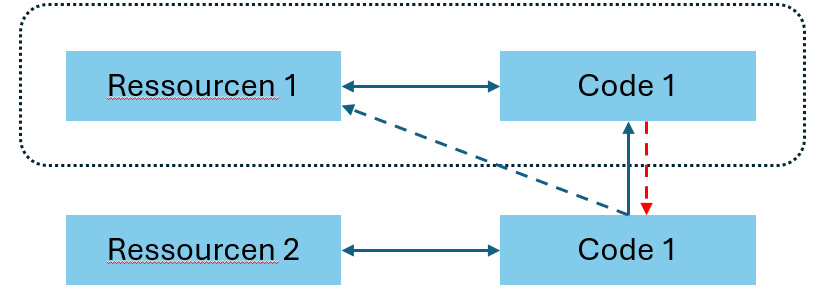
\includegraphics[width=\linewidth]{Grafiken/Sandbox.png}
    \caption{Beschreibung deiner Abbildung hier.}
    \label{fig:sandbox}
\end{figure}
\begin{figure}[h]
    \centering
    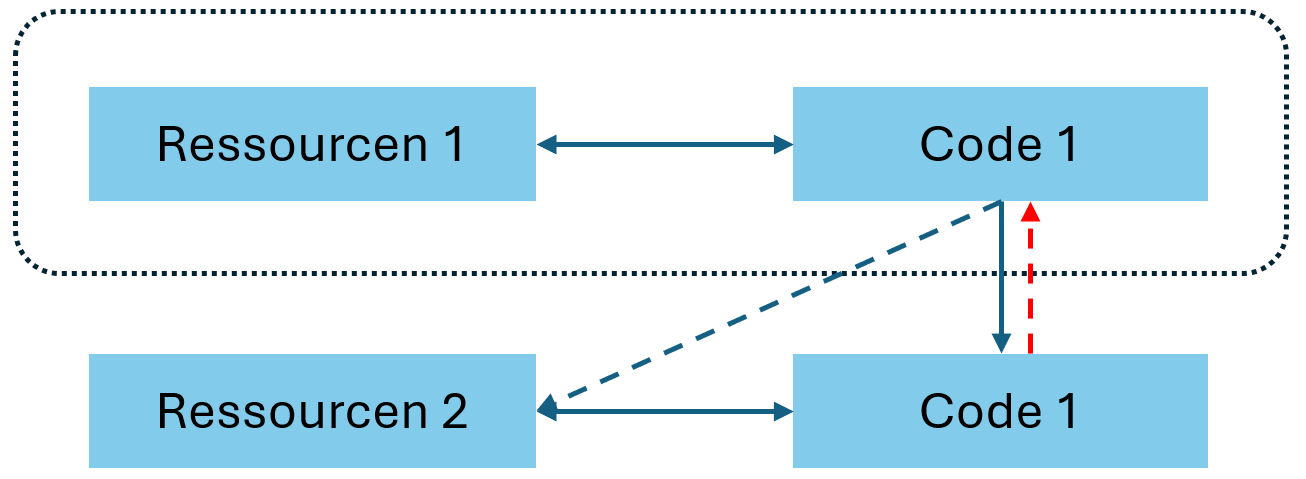
\includegraphics[width=\linewidth]{Grafiken/Safebox.png}
    \caption{Beschreibung deiner Abbildung hier.}
    \label{fig:Safebox}
\end{figure}
\begin{figure}[h]
    \centering
    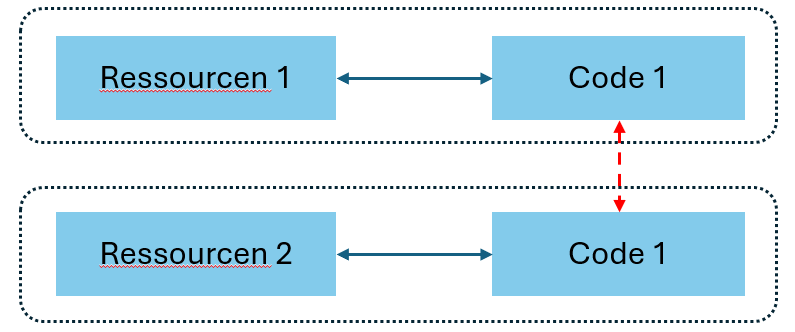
\includegraphics[width=\linewidth]{Grafiken/Kompartiment.png}
    \caption{Beschreibung deiner Abbildung hier.}
    \label{fig:Kompartment}
\end{figure}

